\documentclass[a4paper]{article}

\title{PH2255 Course:\\
Introduction to Statistical Methods\\Exercise 4}
\author{Thomas Bass}
\date{22 January 2021}

% LaTeX preambule: loading relevant packages, configuring Python listings
\usepackage{graphicx}
\usepackage{amsmath}
\usepackage{color}
\usepackage{listings}
\usepackage{hyperref}
\usepackage{bm}
\usepackage{amssymb}

\definecolor{dkgreen}{rgb}{0,0.6,0}
\definecolor{gray}{rgb}{0.5,0.5,0.5}
\definecolor{mauve}{rgb}{0.58,0,0.82}

% Settings for colour-coding and formatting Python code:
\lstset{
  language=Python,                % the language of the code
  basicstyle=\footnotesize,           % the size of the fonts that are used for the code
  numbers=left,                   % where to put the line-numbers
  numberstyle=\tiny\color{gray},  % the style that is used for the line-numbers
  stepnumber=5,                   % the step between two line-numbers. If it's 1, each line
                                  % will be numbered
  numbersep=5pt,                  % how far the line-numbers are from the code
  backgroundcolor=\color{white},      % choose the background color. You must add \usepackage{color}
  showspaces=false,               % show spaces adding particular underscores
  showstringspaces=false,         % underline spaces within strings
  showtabs=false,                 % show tabs within strings adding particular underscores
  frame=single,                   % adds a frame around the code
  rulecolor=\color{black},        % if not set, the frame-color may be changed on line-breaks within not-black text (e.g. commens (green here))
  tabsize=2,                      % sets default tabsize to 2 spaces
  captionpos=b,                   % sets the caption-position to bottom
  breaklines=true,                % sets automatic line breaking
  breakatwhitespace=false,        % sets if automatic breaks should only happen at whitespace
  title=\lstname,                   % show the filename of files included with \lstinputlisting;
                                  % also try caption instead of title
  keywordstyle=\color{blue},          % keyword style
  commentstyle=\color{dkgreen},       % comment style
  stringstyle=\color{mauve},         % string literal style
  escapeinside={\%*}{*)},            % if you want to add LaTeX within your code
  morekeywords={*,...}               % if you want to add more keywords to the set
}

\begin{document}
\maketitle

\subsection{Question 1}
Using Kirchoff's first law to sum the voltages around the LCR circuit:
\begin{equation}
V = IZ = I\left(R+i\omega L+
frac1{i\omega C}\right)
\end{equation}
We can rewrite this in differential form:
\begin{equation}
L\ddot{q}+r\dot{q}+\frac1Cq=0
\end{equation}
This is in the same form as a damped mechanical oscillator $\ddot{q}+\gamma\dot{q}+\omega_0^2q=0$
Therefore $\omega_0=\sqrt{1/LC}$
From definition $\omega=\frac{2\pi}T=2\pi f$
\begin{equation}
f_0=\frac1{2\pi}\sqrt{\frac1{LC}}
\end{equation}

\subsection{Question 2}
Using values of $L=5mH=5\times10^{-3}H$ and $C=1nF=1\times10^{-9}F$:

$f_0=71,176.25Hz$

\subsection{Question 3}
For $\Delta\phi=0$, $f=71.18kHz$

Peak-to-peak voltages:

CH1: $1.463 V$

CH2: $1.082 V$

$\therefore V_2/V_1=0.7395$

This small $$\sim10Hz$$ discrepancy comes from additional impedance from the connections/wires in the circuit.

\subsection{Question 4}

Starting frequency $f_\text{min}=60kHz$, at $V_2/V_1=0.1296$

Ending frequency $f_\text{max}=82kHz$, at $V_2/V_1=0.1357$

\subsection{Question 6}
\begin{equation}
|Z|=\sqrt{R^2+(\omega L-1/\omega C)^2}
\end{equation}

At resonance, $\omega L-1/\omega C=0$, therefore that term drops out of the equation, giving us a minimum value $|Z|=R$.

At high frequencies, the Inductor term $\omega L$ dominates.

At low frequencies, the Capacitor term $1/\omega C$ dominates.

\subsection{Question 7}
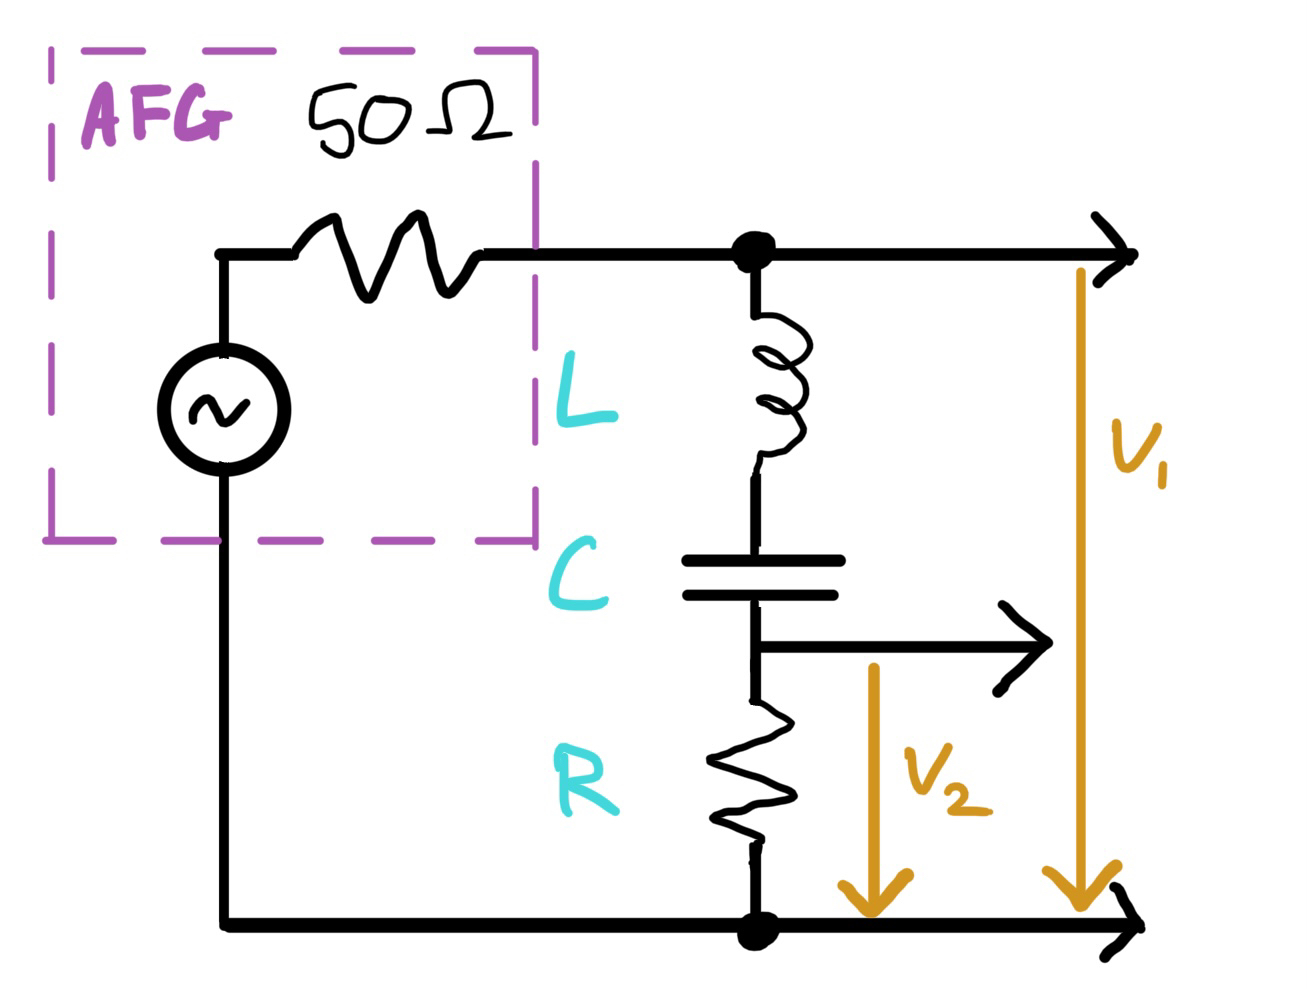
\includegraphics[scale=0.2]{circuit.png}

\subsection{Question 8}
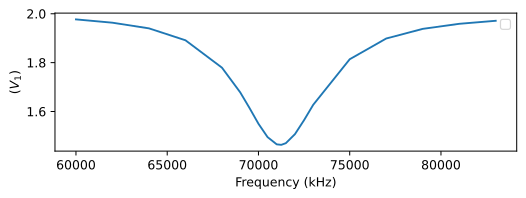
\includegraphics[scale=0.8]{v1.png}

This plot, showing how $V_1$ changes as we change the AFG frequency, takes the form of a $y=\sqrt x$ function. As $V_1$ takes the potential difference over the entire LCR circuit, we include both the resistance, inductance, and capacitance of the three components into account when using Equation 4

\begin{appendix}
\section{Python Code}\label{sec:python}
%\lstinputlisting[language=Python,frame=single]{py.py}%

\end{appendix}

\end{document}
